% Krusche comb trace: A = AB, B = ABBA (m=2, n=4).
% Black-and-white only. Match = solid diagonal, mismatch = dashed diagonal.
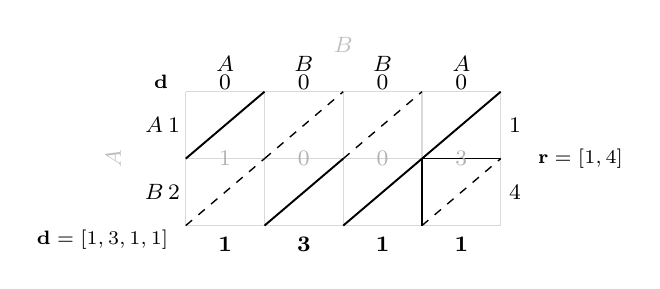
\begin{tikzpicture}[
    matchedge/.style={black, line width=0.7pt},
    missedge/.style={black, line width=0.5pt, dashed},
    swapedge/.style={black, line width=0.5pt},
    gridline/.style={gray!30, thin},
    vallabel/.style={font=\footnotesize},
    strlabel/.style={font=\footnotesize\itshape},
]

\def\cw{1.0}   % cell width
\def\cy{0.85}   % cell height

% ── Grid ────────────────────────────────────────────────────
\draw[gridline] (0, 0) grid[xstep=\cw, ystep=\cy] ({4*\cw}, {2*\cy});

% ── Cell diagonals ──────────────────────────────────────────
% Match cells (r=0,c=0), (r=0,c=3), (r=1,c=1), (r=1,c=2): solid diagonal
\foreach \r/\c in {0/0, 0/3, 1/1, 1/2} {
    \pgfmathsetmacro{\px}{\c*\cw}
    \pgfmathsetmacro{\py}{(1-\r)*\cy}
    \draw[matchedge] (\px, \py) -- +({\cw}, {\cy});
}

% Mismatch cells (no swap): dashed diagonal
\foreach \r/\c in {0/1, 0/2, 1/0} {
    \pgfmathsetmacro{\px}{\c*\cw}
    \pgfmathsetmacro{\py}{(1-\r)*\cy}
    \draw[missedge] (\px, \py) -- +({\cw}, {\cy});
}

% Mismatch-swap cell (r=1, c=3): crossing — vertical + horizontal
\draw[swapedge] ({3*\cw}, 0) -- +({0}, {\cy});
\draw[swapedge] ({3*\cw}, {\cy}) -- +({\cw}, {0});
\draw[missedge] ({3*\cw}, 0) -- +({\cw}, {\cy});

% ── String labels ───────────────────────────────────────────
% Reference B on top
\node[strlabel] at ({0.5*\cw}, {2*\cy + 0.35}) {$A$};
\node[strlabel] at ({1.5*\cw}, {2*\cy + 0.35}) {$B$};
\node[strlabel] at ({2.5*\cw}, {2*\cy + 0.35}) {$B$};
\node[strlabel] at ({3.5*\cw}, {2*\cy + 0.35}) {$A$};
\node[font=\footnotesize, gray!50] at ({2*\cw}, {2*\cy + 0.6}) {$B$};

% Query A on left
\node[strlabel] at (-0.4, {1.5*\cy}) {$A$};
\node[strlabel] at (-0.4, {0.5*\cy}) {$B$};
\node[font=\footnotesize, gray!50, rotate=90, anchor=south] at (-0.7, {\cy}) {$A$};

% ── d_col values at boundaries ──────────────────────────────
% Top: initial d_col = [0, 0, 0, 0]
\foreach \c/\v in {0/0, 1/0, 2/0, 3/0} {
    \node[vallabel] at ({\c*\cw + 0.5*\cw}, {2*\cy + 0.12}) {\v};
}

% Between rows: d_col after row 0 = [1, 0, 0, 3]
\foreach \c/\v in {0/1, 1/0, 2/0, 3/3} {
    \node[vallabel, gray!60] at ({\c*\cw + 0.5*\cw}, {\cy}) {\v};
}

% Bottom: final d_col = [1, 3, 1, 1]
\foreach \c/\v in {0/1, 1/3, 2/1, 3/1} {
    \node[vallabel, font=\footnotesize\bfseries, below]
        at ({\c*\cw + 0.5*\cw}, -0.02) {\v};
}

% d_col label
\node[font=\scriptsize, anchor=east] at (-0.1, {2*\cy + 0.12})
    {$\mathbf{d}$};
\node[font=\scriptsize, anchor=east] at (-0.1, -0.18)
    {$\mathbf{d} = [1,3,1,1]$};

% ── d_row values at boundaries ──────────────────────────────
% Left: initial d_row = [1, 2]
\node[vallabel] at (-0.15, {1.5*\cy}) {$1$};
\node[vallabel] at (-0.15, {0.5*\cy}) {$2$};

% Right: final d_row = [1, 4]
\node[vallabel, font=\footnotesize\bfseries]
    at ({4*\cw + 0.18}, {1.5*\cy}) {$1$};
\node[vallabel, font=\footnotesize\bfseries]
    at ({4*\cw + 0.18}, {0.5*\cy}) {$4$};

% d_row label
\node[font=\scriptsize, anchor=west] at ({4*\cw + 0.35}, {\cy})
    {$\mathbf{r} = [1,4]$};

\end{tikzpicture}
